\documentclass{report}
\usepackage{graphicx} % Required for inserting images
\usepackage[italian]{babel}
\usepackage{tikz}
\usepackage{hyperref}
\usepackage{amsmath}
\usepackage{xcolor}
\usepackage{float}
\usepackage{soul}
\usepackage{listings} % Per evidenziare il codice

\definecolor{lightgray}{rgb}{0.9,0.9,0.9} % Definizione colore sfondo
\definecolor{darkgreen}{rgb}{0.0, 0.5, 0.0}

\lstset{
    backgroundcolor=\color{lightgray}, % Sfondo grigio
    basicstyle=\ttfamily, % Font monospaziato
    % frame=single, % Bordo attorno al codice
    tabsize=4, % Dimensione tabulazione
    breaklines=true, % Permette di andare a capo automaticamente
    numbers = left,
    numberstyle=\small\color{gray}
}

\title{\huge\textbf{{Differential Privacy}}}
\date{Parte IV}
\begin{document}

\maketitle
\tableofcontents
\newpage


\noindent Introdotto nel 2006, ha avuto un'esplosione di utilizzo di questo concetto negli ultimi anni.

\noindent L'idea è la protezione dei dati, i dati sono privati e non basta che siano semplicemente anonimizzati.


\chapter{Basic Scenario}
\begin{figure}[H]
        \centering
        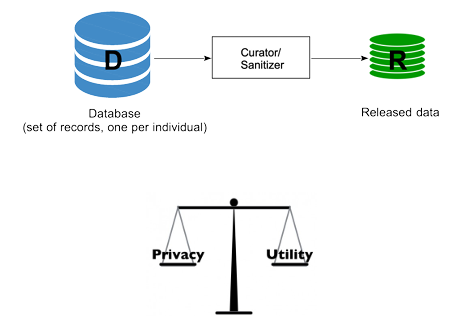
\includegraphics[width=0.6\linewidth]{images/basicScenario.png}
    \end{figure}

\begin{enumerate}
    \item \textbf{D:} Bisogna avere molti dati (se no D.P. non funziona bene), pensiamo di avere tanti record e ciascun record riguarda dati sensibili di individui.
    \item \textbf{Curator/Sanitizer:} è una parte fidata che può accedere in chiaro ai dati
    \item \textbf{R:} Dati rilasciati 
\end{enumerate}

\section{L'intuizione classica per la privacy}
Cosa vuol dire mantenere la privacy degli individui?
\begin{itemize}
    \item Ciò che viene rilasciato non dipende dai miei dati
    \item le informazioni apprese su un individuo dai risultati pubblicati R non sono più di quelle che possiamo apprendere su quell'individuo senza avere accesso a R.
\end{itemize}

\noindent \textbf{Problema:} Se gli individui non hanno impatto sui risultati allora i risultati non avrebbero utilità, serve equilibrio.

\section{Differential privacy– Intuition}
Quello che cerca di fare D.P. è che la presenza o l'assenza di un utente non cambi di molto il rischio di compromettere la sua privacy.
Chiaramente il rilascio di informazioni impone che un minimo cambiamento ci sia, però sia minimale.
Le inferenze che io posso fare su un individuo da un rilascio R deve essere lo stesso che io posso inferire utilizzando i dati di qualunque altro utente.
\begin{figure}[H]
        \centering
        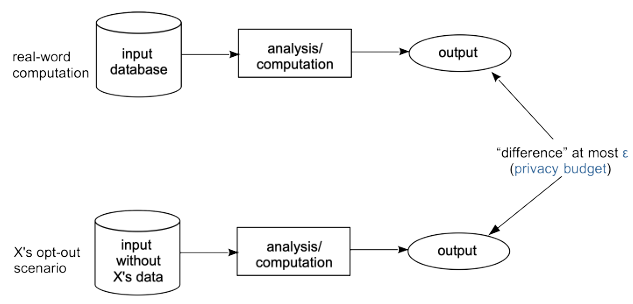
\includegraphics[width=0.6\linewidth]{images/intuition.png}
    \end{figure}

\noindent Più questo $\epsilon$ è piccolo più la differenza dei dati con o senza un determinato individuo è minimale.
Tutto questo viene fatto iniettando del rumore all'interno della mia computazione. Deve essere rumore casuale (NON deterministico)

\noindent Due principali complicazioni:
\begin{itemize}
    \item Capire quanto rumore iniettare
    \item Il risultato della computazione eseguita più volte sullo stesso dataset è sempre diverso, poichè ogni volta viene inserita una quantità di rumore diversa (se viene eseguita la stessa computazione troppe volte si riesce a inferire il valore corretto, da questo nasce
    la necessità del \textbf{Privacy budget})
\end{itemize}

\section{Definizione formale di Differential Privacy}
\textit{Siano due database $D$ e $D'$ due databse vicini (differiscono per un singolo individuo)}
\begin{center}
   \textit{Un algoritmo A soddisfa $\epsilon$-Differential Privacy se per tutte le coppie di database vicini
   $D$, $D'$, e per tutti  gli outputs $o$:}
   
   $P[A(D)= o <= e^\epsilon ]$ $P[A(D')= o]$ 
\end{center}

\textbf{N.B.:} 
\begin{itemize}
    \item La definizione si riferisce a una computazione (non ai dati) quindi ad un algoritmo A, ed è l'algoritmo che soddisfa la definizone di D.P.
    \item D.P. è soddisfatta quando qualunque sia la coppia di dataset $D$ e $D'$ che vengono considerati (basta che siano vicini), quando applicando
    una determinata computazione su $D$, la probabilità di ottenere un determinato risultato più o meno deve essere uguale alla probabilità di ottenere lo stesso
    risultato applicando lo stesso algoritmo su $D'$
    \item La variazione dipende da questo parametro $\epsilon$
    \item Per un attaccante è impossibile capire se un determinato risultato viene prodotto da $D$ o da $D'$
    \item Tutto questo funziona bene se abbiamo grandi quantità di dati, se sono piccole si rischia di dover inserire troppo rumore e che i dati non siano più utili
\end{itemize}

\section{Pivacy budget $\epsilon$}
Determina quanto  \textbf{rumore} viene inserito nella computazione, un trade-off tra utilità e privacy.
\begin{itemize}
    \item \textbf{piccolo $\epsilon$:} più privacy, meno utilità
    \item \textbf{grande $\epsilon$:} meno privacy, più utilità
\end{itemize}

\noindent Se $\epsilon = 0$ allora avremmo due distribuzioni di probabilità esattamente identiche
avremmo la privacy maggiore in assoluto, ma bassissima utilità dei dati poichè il risultato della computazione non dipenderebbe dai dati di nessun indviduo (quindi non dipende dall'input, risultato casuale).
Man mano che $\epsilon$ aumenta aumenta anche la diversità e quindi l'impatto di ogni singolo individuo, minore privacy ma maggiore utilità.
Il miglior valore di $\epsilon$ non si sa con certezza, si considerano buoni valori di $\epsilon$ valori minori di uno. 
\begin{figure}[H]
        \centering
        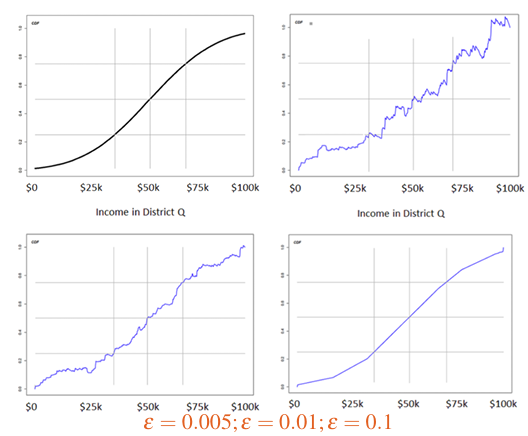
\includegraphics[width=0.4\linewidth]{images/curve.png}
    \end{figure}

\section{Global sensitivity}
Il problema di questa tecnica è capire quanto rumore inserire nel risultato della computazione per garantire il soddisfacimento della definizione,
l'idea è quella di calibrare la quantità di rumore sulla base di qual è l'influenza sui dati di un singolo individuo sul risultato della computazione.

\begin{itemize}
    \item \textbf{Sensitività globale:} caratterizza l'entità dell'influenza di un singolo individuo (caso peggiore), e quindi la quantità di rumore che si deve aggiungere 
\end{itemize}

\subsubsection{Esempio 1(scelto anche esempio di conteggio poichè sono quelli che funzionano meglio con questa tecnica)}

\noindent Supponiamo di avere questi dati da un ospedale e di voler calcolare quanti pazienti hanno l'influenza:
\begin{figure}[H]
        \centering
        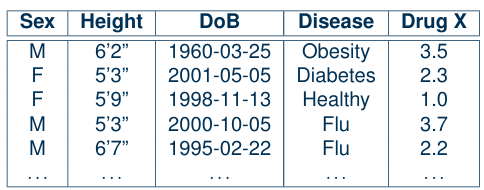
\includegraphics[width=0.4\linewidth]{images/pazienti.png}
    \end{figure}
\noindent Immaginiamo che nel DB $D$ ci sono 50 pazienti con l'influenza, bisogna capire quanto rumore iniettare per soddisfare D.P.
Togliendo uno qualunque dei 50 pazienti ne avremmo 49, quindi noi vogliamo mascherare il fatto che anche solo togliendone uno questo ha un impatto.


\noindent Nel caso peggiore il nostro impatto è pari a 1, se uno di questi individui con influenza c'è abbiamo 50 pazienti, se no sono 49.

\noindent Per questo motivo in questo esempio la \textbf{global sensitivity} è pari a 1.

\noindent Per qualsiasi tipo di conteggio la global sensitivity sarà sempre 1. 

\subsubsection{Esempio 2 (sulla stessa tabella)}

\noindent Supponiamo di voler calcolare la somma di quanto di un determinato mediciale è stato somministrato ai pazienti. In questo caso la global sensitivity, togliendo i dati di un individuo, raramente sarà pari a 1. Inoltre noi vogliamo stimare il \textbf{caso peggiore}.

\noindent Avendo solo i pazienti visibili in tabella, il paziente numero 4 sarebbe il caso peggiore ossia la G.S. sarebbe pari a 3.7, ma nel caso in cui venisse aggiunto un nuovo paziente
più impattante la G.S. cambierebbe quindi non è semplice capire come calcolare la G.S, questo esempio per capire che già per una computazione piccola è difficile stimarla.

\noindent Nella slide infatti viene assunto che i valori di questo medicinale possono essere compresi solamente tra 1 e 4, in questo modo calcoare il caso peggiore è semplificato.

\section{Tecniche di generazione di rumore}
Per esempio si può usare la Distribuzione di Laplace, caratterizzata dal parametro $\lambda$ che nel nostro caso 
è ottenuto come Global sensitivity/$\epsilon$

\begin{figure}[H]
        \centering
        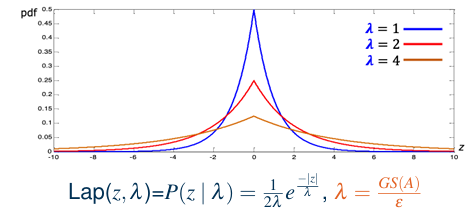
\includegraphics[width=0.4\linewidth]{images/Laplace.png}
    \end{figure}
\noindent Più è grande la Global sensitivity più è grande $\lambda$ ed è inversamente proporzionale ad $\epsilon$ 
\begin{itemize}
    \item \textbf{$\lambda$ = 1:} alta probabilità di aggiungere una piccola quantità di rumore, l'area maggiore è nell'intorno dello zero
    \item \textbf{$\lambda$ aumenta:} più lambda aumenta più le curve sono flat, sopratutto allontanandosi dallo zero. Quindi più $\lambda$ è grande maggiore sarà la probabilità di aggiungere tanto rumore 
\end{itemize}

\section{Global picture}
Mettiamo insieme tutto:
\begin{figure}[H]
        \centering
        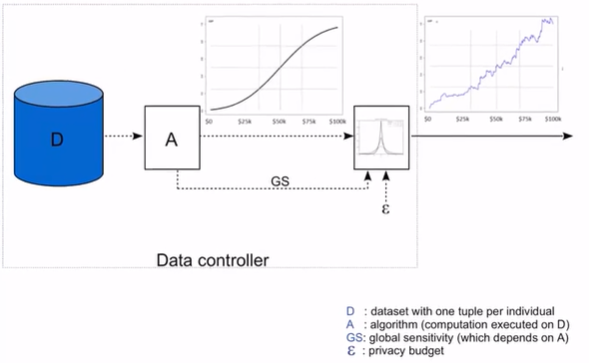
\includegraphics[width=0.6\linewidth]{images/slideextra.png}
    \end{figure}
\noindent Applicare Differential privacy vuol dire:
\begin{enumerate}
    \item Parto da una collezione di dati $D$, contenenti informazioni sensibili
    \item Sui quali vogliamo eseguire una computazione $A$
    \item In base alla computazione che vogliamo eseguire calcoliamo la Global sensitivity
    \item Applico la computazione $A$ sullla collezione di dati $D$, ottengo il risultato
    \item Sporco il risultato con il \textbf{rumore} applicando delle tecniche tipo quella di Laplace
    \item Restituisco il  risultato sporcato
\end{enumerate}

\chapter{Proprietà di Differential Privacy}
\section{Chiusura del post-processing}
Resiliente a operazioni di post-procesing.

\noindent C'è una fase di post-processing da fare sui risultati aggiunti di rumore prima di rilasciarli.

\noindent \textbf{Questa proprietà ci dice che non vi è differenza tra i risultati prima e dopo il post-processing,
entrambi rispettano la proprietà di Differential Privacy}
\begin{figure}[H]
        \centering
        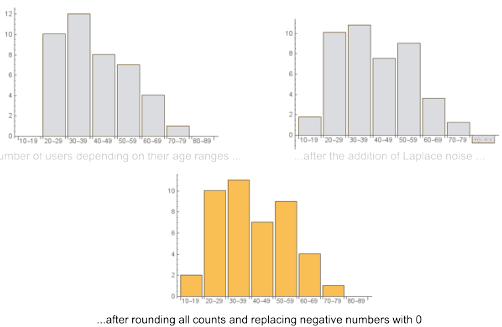
\includegraphics[width=0.4\linewidth]{images/postP.png}
\end{figure}

\section{Composizione parallela}
\begin{center}
    \textit{"Differential privacy si compone bene con se stessa" ma cosa vuol dire?}
\end{center}
\noindent \textbf{Composizione parallela:} sequenza di $m$ computazioni su sottoinsiemi disgiunti di una base di dati $D$

\begin{figure}[H]
        \centering
        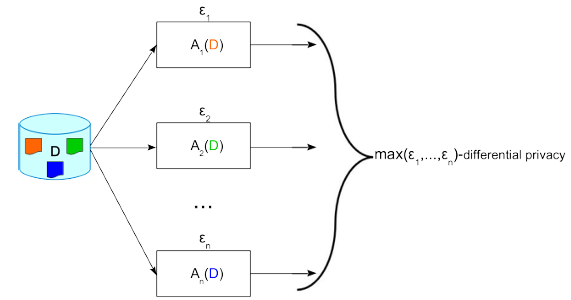
\includegraphics[width=0.4\linewidth]{images/ParallelC.png}
\end{figure}


\noindent Da una parte abbiamo i dati $D$, a bbiamo tante computazioni fatte su questi dati. Successivamente i risultati di queste computazioni vengono rilasciate
(sempre sugli stessi dati), rilasciando più computazioni è sempre più probabile inferire qualcosa sui dati iniziali.

\noindent Con D.P. possiamo quantificare precisamente quanto varia la privacy degli individui ma mano che rilascio i risultati delle computaioni, e posso definirlo in modo preciso:

\noindent \textbf{Se io eseguo varie computazioni so precisamente quali parte del DB vanno a toccare, quindi è vero che eseguo $m$ computazioni ma non è detto che ci siano intersezioni tra di esse.
Tutte le informazioni sono protette con un $\epsilon$ che è il massimo degli $\epsilon$ che è stato usato}

\section{Composizione sequenziale}
\noindent \textbf{Composizione sequanziale:} sequenza di $m$ computazioni su database $D$ con risultati sovrapposti

\begin{figure}[H]
        \centering
        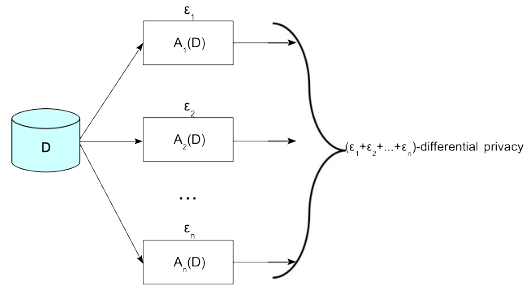
\includegraphics[width=0.4\linewidth]{images/sequenziale.png}
\end{figure}

\noindent La differenza rispetto al caso precedente è che riguardano individui non disgiunti, più computazioni sugli stessi individui.

\noindent \textbf{In questo caso rilasciare tutte queste informazioni equivale a rilasciarne una contenente tutte le informazioni, e $\epsilon$ verrà calcolato sommando i singoli $\epsilon$
utilizzati nelle singole computazioni}

\newpage
\section{Perchè $\epsilon$ è chiamato "Privacy budget"?}
$\epsilon$ rappresenta il livello di protezione che voglio mantenere, ogni volta che eseguo una computazione, è come se utilizzassi parte di questo budget.

\noindent Quando il budget si esuarisce, non posso più eseguire computazioni poichè ho raggiunto l' $\epsilon$ che mi ero prefissato
\begin{figure}[H]
        \centering
        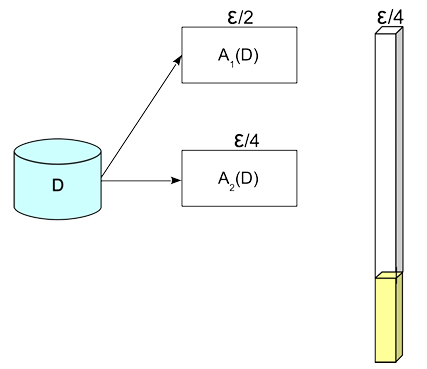
\includegraphics[width=0.4\linewidth]{images/privacyBudget.png}
\end{figure}

\chapter{Modelli di Differential Privacy}

\section{Interattivo VS non Interattivo}
\begin{figure}[H]
        \centering
        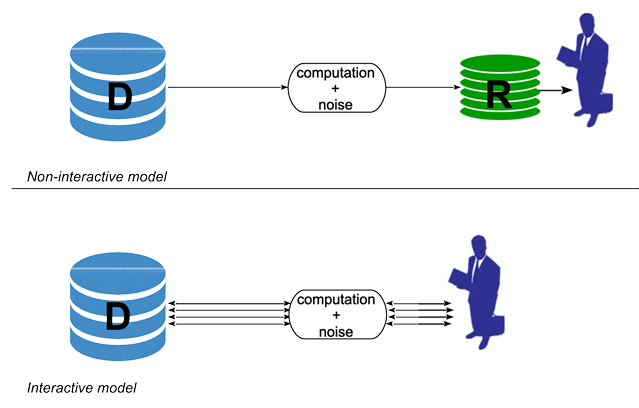
\includegraphics[width=0.3\linewidth]{images/Interactive.png}
\end{figure}
\begin{itemize}
    \item \textbf{Interattivo:} valutazione delle query run-time 
    \item \textbf{Non interattivo:} chi ha in mano i dati decide cosa rilasciare a priori, rilascio di dati pre-computati in macrotabelle 
\end{itemize}


\section{Globale VS Locale}
\begin{figure}[H]
        \centering
        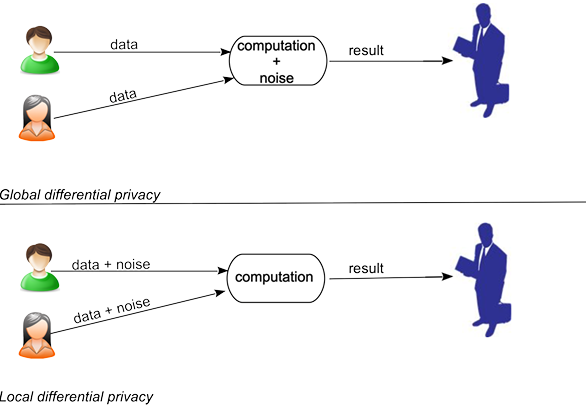
\includegraphics[width=0.3\linewidth]{images/Gloabl.png}
\end{figure}
\begin{itemize}
    \item \textbf{Globale:} c'è un'entità fidata che esegue la computazione sui dati proteggendo il risultato della computazione con differential privacy
    \item \textbf{Locale:} non c'è più una parte fidata che riceve i dati degli utenti, c'è qualcuno che colleziona i dati ma non essendo fidato non riceve i dati originale ma dati già sporcat di rumore
\end{itemize}

\subsection{Definizione formale di Local Differential Privacy}
\textit{Un algoritmo randomizzato $K$ soddisfa $\epsilon$-local differential privacy
se e solo se per ogni input $x$,$x'$ e output $o$ di $A$:}
\begin{center}
    \textit{$P[K(x) = o]<= e^\epsilon$ $P[K(x') = o]$}
\end{center}

\noindent Al posto di avere $D$ e $D'$ che sono collezioni di dati, ma sono i dati di un individuo, tutto il resto si applica allo stesso modo della Global.

\chapter{Differential Privacy nel mondo reale}
\section{Privacy in practice}
Differential privacy basata sul \textbf{Lancio della moneta} molto usata in Google e Apple.

\noindent si basa sull'idea di lanciare la moneta
\begin{figure}[H]
        \centering
        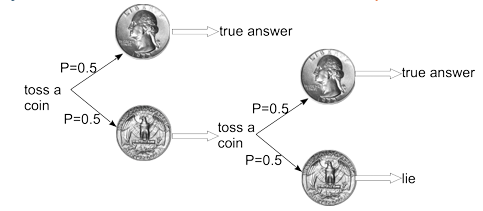
\includegraphics[width=0.3\linewidth]{images/coin.png}
\end{figure}
\noindent Questo stesso meccanismo è usato per proteggere la privacy dei miei dati prima che finiscano in mano alla terza parte non fidata,
viene protetto ogni singolo bit in questo modo. 

\noindent La protezione ottenuta è pari a $\epsilon = ln(3)$

\section{Esempio dei censimenti}
L'Ufficio del Censimento degli Stati Uniti ha distribuito OnTheMap, un'applicazione basata sul web che mostra dove i lavoratori sono occupati e dove vivono.

\noindent E' basato su un'idea diversa di differential privacy, ovvero:
\begin{center}
    \textit{$(\epsilon, \delta)$-differential privacy}
\end{center}

\begin{itemize}
    \item $\epsilon$ è il privacy budget
    \item $\delta$ ci dice quanto il risultato rilasciato è maggiore rispetto all'$\epsilon$ che mi ero prefissato
\end{itemize}

\chapter{Problemi con differential privacy}
Ha rivoluzionato molto ma ha anche delle problematiche:
\begin{itemize}
    \item Finchè si tratta di conteggi va tutto molto bene, ma con altre computazioni è difficile stabilire la global sensitivity
    \item A volte viene inserito troppo rumore per proteggere gli outlier 
    \item Come settare il valore di $\epsilon$, viene suggerita la soluzione che quando il privacy budget è esaurito allora le computazioni verranno eseguire su dati sintetici(difficile)
\end{itemize}







\end{document}